% Options for packages loaded elsewhere
\PassOptionsToPackage{unicode}{hyperref}
\PassOptionsToPackage{hyphens}{url}
%
\documentclass[
]{article}
\usepackage{amsmath,amssymb}
\usepackage{lmodern}
\usepackage{iftex}
\ifPDFTeX
  \usepackage[T1]{fontenc}
  \usepackage[utf8]{inputenc}
  \usepackage{textcomp} % provide euro and other symbols
\else % if luatex or xetex
  \usepackage{unicode-math}
  \defaultfontfeatures{Scale=MatchLowercase}
  \defaultfontfeatures[\rmfamily]{Ligatures=TeX,Scale=1}
\fi
% Use upquote if available, for straight quotes in verbatim environments
\IfFileExists{upquote.sty}{\usepackage{upquote}}{}
\IfFileExists{microtype.sty}{% use microtype if available
  \usepackage[]{microtype}
  \UseMicrotypeSet[protrusion]{basicmath} % disable protrusion for tt fonts
}{}
\makeatletter
\@ifundefined{KOMAClassName}{% if non-KOMA class
  \IfFileExists{parskip.sty}{%
    \usepackage{parskip}
  }{% else
    \setlength{\parindent}{0pt}
    \setlength{\parskip}{6pt plus 2pt minus 1pt}}
}{% if KOMA class
  \KOMAoptions{parskip=half}}
\makeatother
\usepackage{xcolor}
\usepackage[margin=1in]{geometry}
\usepackage{color}
\usepackage{fancyvrb}
\newcommand{\VerbBar}{|}
\newcommand{\VERB}{\Verb[commandchars=\\\{\}]}
\DefineVerbatimEnvironment{Highlighting}{Verbatim}{commandchars=\\\{\}}
% Add ',fontsize=\small' for more characters per line
\usepackage{framed}
\definecolor{shadecolor}{RGB}{248,248,248}
\newenvironment{Shaded}{\begin{snugshade}}{\end{snugshade}}
\newcommand{\AlertTok}[1]{\textcolor[rgb]{0.94,0.16,0.16}{#1}}
\newcommand{\AnnotationTok}[1]{\textcolor[rgb]{0.56,0.35,0.01}{\textbf{\textit{#1}}}}
\newcommand{\AttributeTok}[1]{\textcolor[rgb]{0.77,0.63,0.00}{#1}}
\newcommand{\BaseNTok}[1]{\textcolor[rgb]{0.00,0.00,0.81}{#1}}
\newcommand{\BuiltInTok}[1]{#1}
\newcommand{\CharTok}[1]{\textcolor[rgb]{0.31,0.60,0.02}{#1}}
\newcommand{\CommentTok}[1]{\textcolor[rgb]{0.56,0.35,0.01}{\textit{#1}}}
\newcommand{\CommentVarTok}[1]{\textcolor[rgb]{0.56,0.35,0.01}{\textbf{\textit{#1}}}}
\newcommand{\ConstantTok}[1]{\textcolor[rgb]{0.00,0.00,0.00}{#1}}
\newcommand{\ControlFlowTok}[1]{\textcolor[rgb]{0.13,0.29,0.53}{\textbf{#1}}}
\newcommand{\DataTypeTok}[1]{\textcolor[rgb]{0.13,0.29,0.53}{#1}}
\newcommand{\DecValTok}[1]{\textcolor[rgb]{0.00,0.00,0.81}{#1}}
\newcommand{\DocumentationTok}[1]{\textcolor[rgb]{0.56,0.35,0.01}{\textbf{\textit{#1}}}}
\newcommand{\ErrorTok}[1]{\textcolor[rgb]{0.64,0.00,0.00}{\textbf{#1}}}
\newcommand{\ExtensionTok}[1]{#1}
\newcommand{\FloatTok}[1]{\textcolor[rgb]{0.00,0.00,0.81}{#1}}
\newcommand{\FunctionTok}[1]{\textcolor[rgb]{0.00,0.00,0.00}{#1}}
\newcommand{\ImportTok}[1]{#1}
\newcommand{\InformationTok}[1]{\textcolor[rgb]{0.56,0.35,0.01}{\textbf{\textit{#1}}}}
\newcommand{\KeywordTok}[1]{\textcolor[rgb]{0.13,0.29,0.53}{\textbf{#1}}}
\newcommand{\NormalTok}[1]{#1}
\newcommand{\OperatorTok}[1]{\textcolor[rgb]{0.81,0.36,0.00}{\textbf{#1}}}
\newcommand{\OtherTok}[1]{\textcolor[rgb]{0.56,0.35,0.01}{#1}}
\newcommand{\PreprocessorTok}[1]{\textcolor[rgb]{0.56,0.35,0.01}{\textit{#1}}}
\newcommand{\RegionMarkerTok}[1]{#1}
\newcommand{\SpecialCharTok}[1]{\textcolor[rgb]{0.00,0.00,0.00}{#1}}
\newcommand{\SpecialStringTok}[1]{\textcolor[rgb]{0.31,0.60,0.02}{#1}}
\newcommand{\StringTok}[1]{\textcolor[rgb]{0.31,0.60,0.02}{#1}}
\newcommand{\VariableTok}[1]{\textcolor[rgb]{0.00,0.00,0.00}{#1}}
\newcommand{\VerbatimStringTok}[1]{\textcolor[rgb]{0.31,0.60,0.02}{#1}}
\newcommand{\WarningTok}[1]{\textcolor[rgb]{0.56,0.35,0.01}{\textbf{\textit{#1}}}}
\usepackage{graphicx}
\makeatletter
\def\maxwidth{\ifdim\Gin@nat@width>\linewidth\linewidth\else\Gin@nat@width\fi}
\def\maxheight{\ifdim\Gin@nat@height>\textheight\textheight\else\Gin@nat@height\fi}
\makeatother
% Scale images if necessary, so that they will not overflow the page
% margins by default, and it is still possible to overwrite the defaults
% using explicit options in \includegraphics[width, height, ...]{}
\setkeys{Gin}{width=\maxwidth,height=\maxheight,keepaspectratio}
% Set default figure placement to htbp
\makeatletter
\def\fps@figure{htbp}
\makeatother
\setlength{\emergencystretch}{3em} % prevent overfull lines
\providecommand{\tightlist}{%
  \setlength{\itemsep}{0pt}\setlength{\parskip}{0pt}}
\setcounter{secnumdepth}{-\maxdimen} % remove section numbering
\ifLuaTeX
  \usepackage{selnolig}  % disable illegal ligatures
\fi
\IfFileExists{bookmark.sty}{\usepackage{bookmark}}{\usepackage{hyperref}}
\IfFileExists{xurl.sty}{\usepackage{xurl}}{} % add URL line breaks if available
\urlstyle{same} % disable monospaced font for URLs
\hypersetup{
  pdftitle={PSTAT 131 HW1},
  pdfauthor={Lishan Shi},
  hidelinks,
  pdfcreator={LaTeX via pandoc}}

\title{PSTAT 131 HW1}
\author{Lishan Shi}
\date{2022-10-01}

\begin{document}
\maketitle

Machine Learning Main Ideas Please answer the following questions. Be
sure that your solutions are clearly marked and that your document is
neatly formatted.

You don't have to rephrase everything in your own words, but if you
quote directly, you should cite whatever materials you use (this can be
as simple as ``from the lecture/page \# of book'').

\textbf{Question 1:} Define supervised and unsupervised learning. What
are the difference(s) between them?

\textbf{Supervised learning:} We are interested in how to accurately
predict future response using given predictors. In other words, we are
trying to understand how predictors affect response. In terms of model
selection, we may try multiple different models to predict and find the
best model for response given predictors. From a inference view, we
assess the quality of our predictions and estimation (from lecture).
Supervised statistical learning involves building a statistical model
for predicting, or estimating, an output based on one or more inputs
(ISLR \#1).

\textbf{Unsupervised learning:} In this case, we only have predictors
but not response, which means that there is no answer key for the
prediction (from lecture). With the unsupervised learning, there are
inputs but no supervising output; nevertheless we can learn
relationships and structure from such data. For example, in a marketing
setting, we might have demographic information for a number of current
or potential customers. We may wish to understand which types of
customers are similar to each other by grouping individuals according to
their observed characteristics. This is known as a clustering problem.
Unlike in the supervised learning, here we are not trying to predict an
output variable (ISLR \#1 \& \#4).

The main difference between supervised and unsupervised learning is
whether we have response or not. The goal for supervised learning is to
accurately predict the response based on predictors, whereas for
unsupervised learning, we are no longer interested in prediction but in
the relationship and structure of data.

\textbf{Question 2:} Explain the difference between a regression model
and a classification model, specifically in the context of machine
learning.

The difference between a regression model and a classification model is
whether the output is quantitative or qualitative. For a regression
model, the outputs are continuous or quantitative. For a classification
model, the outputs are qualitative, i.e.~categorical values (from
lecture).

\textbf{Question 3:} Name two commonly used metrics for regression ML
problems. Name two commonly used metrics for classification ML problems.

Regression ML problems: MSE, Variance Classification ML problems: Error
rate, Bayes Error Rate, Bayes classifier,Accuracy etc.

\textbf{Question 4:} As discussed, statistical models can be used for
different purposes. These purposes can generally be classified into the
following three categories. Provide a brief description of each.

Descriptive models: choose model to best visually emphasize a trend in
data

Inferential models: infer significant features of model, state
relationship between outcome \& predictors, aim to test theories, have
possibly causal claims

Predictive models: aim to predict output with minimum reducible error,
not focus on hypothesis tests

\textbf{Question 5:} Predictive models are frequently used in machine
learning, and they can usually be described as either mechanistic or
empirically-driven. Answer the following questions.

Define mechanistic. Define empirically-driven. How do these model types
differ? How are they similar?

\textbf{Mechanistic (Parametric):} Parametric methods involve a two-step
model-based approach. Assume a parametric form for function f, and use
data to train the model. This method, however, would not match true
unknown function f, and may cause overfitting if there are too many
parameters (ISLR \#21).

\textbf{Empirically-driven (non-parametric):} Have no assumption about
function f, require a larger number of observations, are much more
flexible by default, have the potential to accurately fit a wider range
of possible shapes for function f, may also have issue of overfitting
(ISLR \#23).

They are different in the way that mechanistic model assumes the
parametric form of function f in the first place whereas the
empirically-driven model has no assumption of function
f.~Empirically-driven model is thus more flexible than mechanistic
model. However, both models may encounter issue of overfitting.

In general, is a mechanistic or empirically-driven model easier to
understand? Explain your choice.

I personally think that mechanistic model is easier to understand
compared to empirically-driven model, as mechanistic model essentially
reduces the problem of estimating f down to one of estimating a set of
parameters, meaning that the parametric form of the model is assumed in
the first place. I am more familiar with the parametric forms and
parameter estimation compared to the procedure that non-parametric
method has.

Describe how the bias-variance tradeoff is related to the use of
mechanistic or empirically-driven models.

Mechanistic models usually have high bias and low variance since we
assume the parametric form of the model in the first place.
Empirically-driven models, on the other hand, have low bias and high
variance due to the lack of assumption of functional form.

\textbf{Question 6:} A political candidate's campaign has collected some
detailed voter history data from their constituents. The campaign is
interested in two questions:

Given a voter's profile/data, how likely is it that they will vote in
favor of the candidate?

How would a voter's likelihood of support for the candidate change if
they had personal contact with the candidate?

Classify each question as either predictive or inferential. Explain your
reasoning for each.

The first question is predictive because we use the given information of
data to predict the outcome. The second question is inferential because
we are interested in the relationship between the support of the
candidate and personal contact with candidate.

\textbf{Exploratory Data Analysis} This section will ask you to complete
several exercises. For this homework assignment, we'll be working with
the mpg data set that is loaded when you load the tidyverse. Make sure
you load the tidyverse and any other packages you need.

Exploratory data analysis (or EDA) is not based on a specific set of
rules or formulas. It is more of a state of curiosity about data. It's
an iterative process of:

generating questions about data visualize and transform your data as
necessary to get answers use what you learned to generate more questions
A couple questions are always useful when you start out. These are
``what variation occurs within the variables,'' and ``what covariation
occurs between the variables.''

You should use the tidyverse and ggplot2 for these exercises.

\textbf{Exercise 1:} We are interested in highway miles per gallon, or
the hwy variable. Create a histogram of this variable. Describe what you
see/learn.

\begin{Shaded}
\begin{Highlighting}[]
\FunctionTok{library}\NormalTok{(tidyverse)}
\end{Highlighting}
\end{Shaded}

\begin{verbatim}
## -- Attaching packages --------------------------------------- tidyverse 1.3.2 --
## v ggplot2 3.3.6      v purrr   0.3.4 
## v tibble  3.1.8      v dplyr   1.0.10
## v tidyr   1.2.1      v stringr 1.4.1 
## v readr   2.1.2      v forcats 0.5.2 
## -- Conflicts ------------------------------------------ tidyverse_conflicts() --
## x dplyr::filter() masks stats::filter()
## x dplyr::lag()    masks stats::lag()
\end{verbatim}

\begin{Shaded}
\begin{Highlighting}[]
\FunctionTok{ggplot}\NormalTok{(mpg,}\FunctionTok{aes}\NormalTok{(}\AttributeTok{x=}\NormalTok{hwy))}\SpecialCharTok{+}\FunctionTok{geom\_histogram}\NormalTok{()}\SpecialCharTok{+}\FunctionTok{labs}\NormalTok{(}\AttributeTok{x=}\StringTok{"Highway miles per gallon"}\NormalTok{,}\AttributeTok{y=}\StringTok{"Frequency"}\NormalTok{)}
\end{Highlighting}
\end{Shaded}

\begin{verbatim}
## `stat_bin()` using `bins = 30`. Pick better value with `binwidth`.
\end{verbatim}

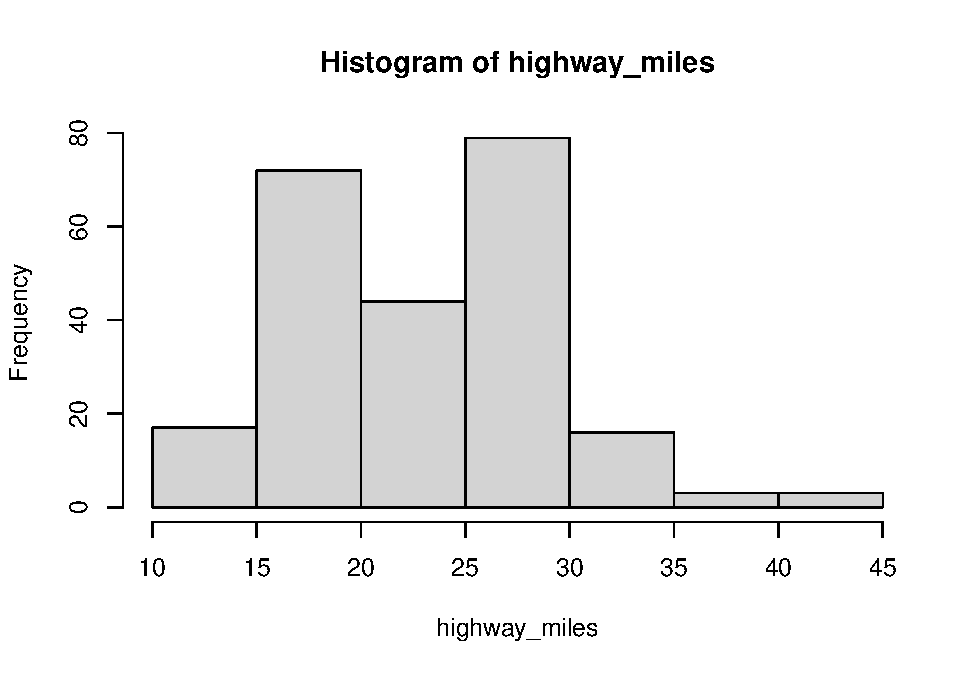
\includegraphics{PSTAT131-HW1_files/figure-latex/unnamed-chunk-1-1.pdf}
I observe that people mostly drive 15 to 30 miles per gallon on highway.
In particular, 25 to 30 miles per gallon has the highest frequency. Only
a few can drive 35 to 45 miles per gallon on highway.

\textbf{Exercise 2:} Create a scatterplot. Put hwy on the x-axis and cty
on the y-axis. Describe what you notice. Is there a relationship between
hwy and cty? What does this mean?

\begin{Shaded}
\begin{Highlighting}[]
\FunctionTok{ggplot}\NormalTok{(mpg,}\FunctionTok{aes}\NormalTok{(}\AttributeTok{x=}\NormalTok{hwy,}\AttributeTok{y=}\NormalTok{cty))}\SpecialCharTok{+}\FunctionTok{geom\_point}\NormalTok{()}\SpecialCharTok{+}\FunctionTok{labs}\NormalTok{(}\AttributeTok{x=}\StringTok{"Highway Miles per Gallon"}\NormalTok{,}\AttributeTok{y=}\StringTok{"City Mileage"}\NormalTok{)}
\end{Highlighting}
\end{Shaded}

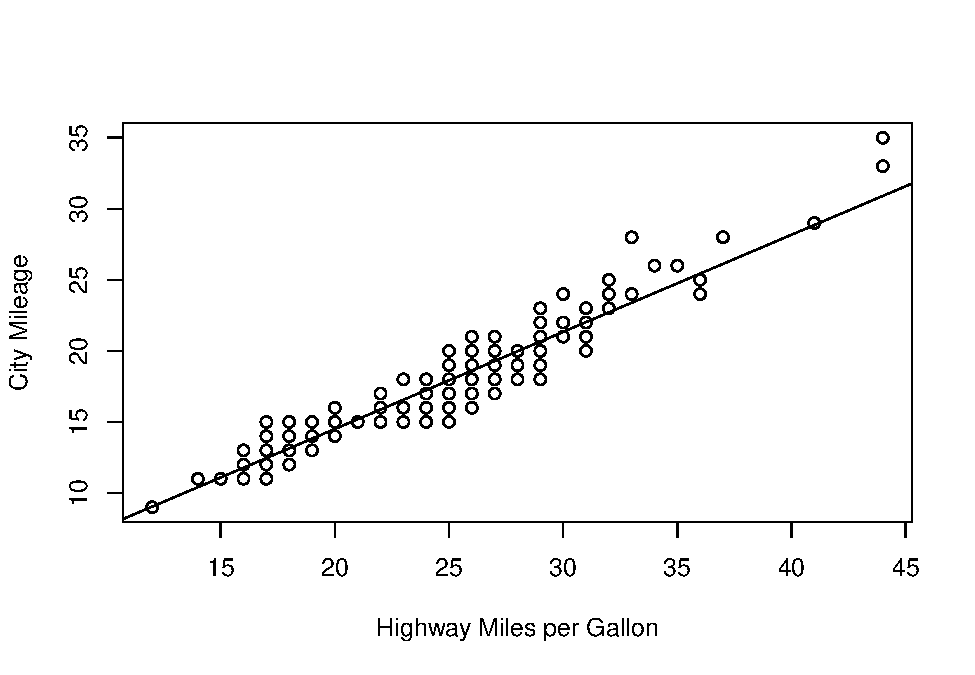
\includegraphics{PSTAT131-HW1_files/figure-latex/unnamed-chunk-2-1.pdf}
I notice that there is a positive linear relationship between highway
miles per gallon and city mileage. This means that as the highway miles
increase, city mileage also increases.

\textbf{Exercise 3:} Make a bar plot of manufacturer. Flip it so that
the manufacturers are on the y-axis. Order the bars by height. Which
manufacturer produced the most cars? Which produced the least?

\begin{Shaded}
\begin{Highlighting}[]
\FunctionTok{ggplot}\NormalTok{(mpg, }\FunctionTok{aes}\NormalTok{(}\AttributeTok{y=}\FunctionTok{reorder}\NormalTok{(}\FunctionTok{factor}\NormalTok{(manufacturer),manufacturer,}\ControlFlowTok{function}\NormalTok{(y)}\SpecialCharTok{{-}}\FunctionTok{length}\NormalTok{(y),}\AttributeTok{decreasing=}\ConstantTok{TRUE}\NormalTok{)))}\SpecialCharTok{+}\FunctionTok{geom\_bar}\NormalTok{() }
\end{Highlighting}
\end{Shaded}

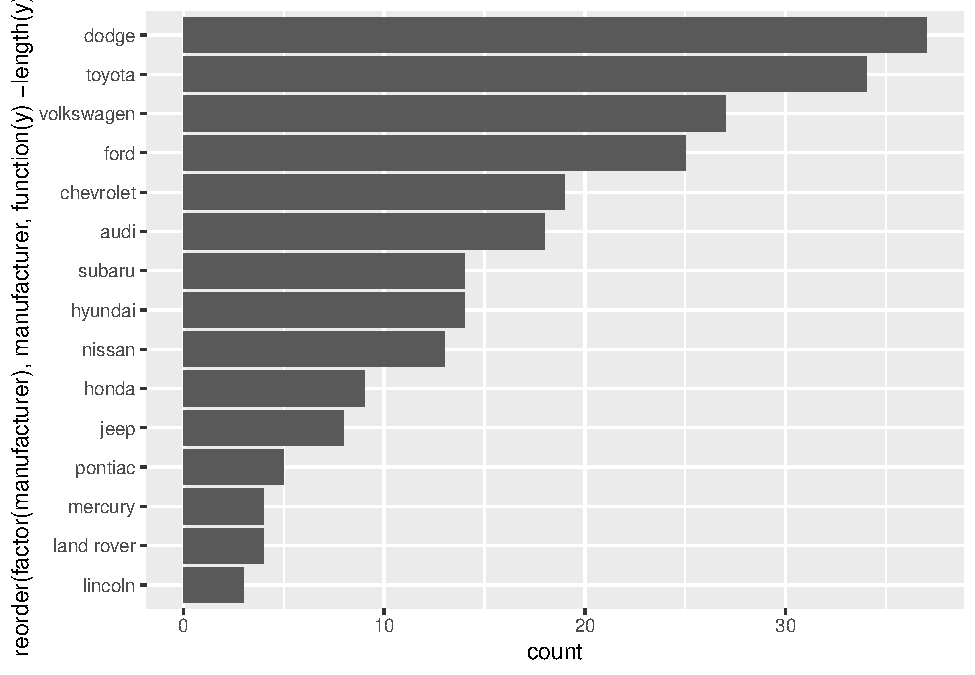
\includegraphics{PSTAT131-HW1_files/figure-latex/unnamed-chunk-3-1.pdf}
Observation: Dodge produced the most cars, whereas lincoln produced the
least cars.

\textbf{Exercise 4:} Make a box plot of hwy, grouped by cyl. Do you see
a pattern? If so, what?

\begin{Shaded}
\begin{Highlighting}[]
\FunctionTok{ggplot}\NormalTok{(mpg,}\FunctionTok{aes}\NormalTok{(}\AttributeTok{x=}\FunctionTok{factor}\NormalTok{(cyl),}\AttributeTok{y=}\NormalTok{hwy))}\SpecialCharTok{+}\FunctionTok{geom\_boxplot}\NormalTok{()}\SpecialCharTok{+}\FunctionTok{labs}\NormalTok{(}\AttributeTok{x=}\StringTok{"Number of Cylinders"}\NormalTok{,}\AttributeTok{y=}\StringTok{"Highway Miles per Gallon"}\NormalTok{)}
\end{Highlighting}
\end{Shaded}

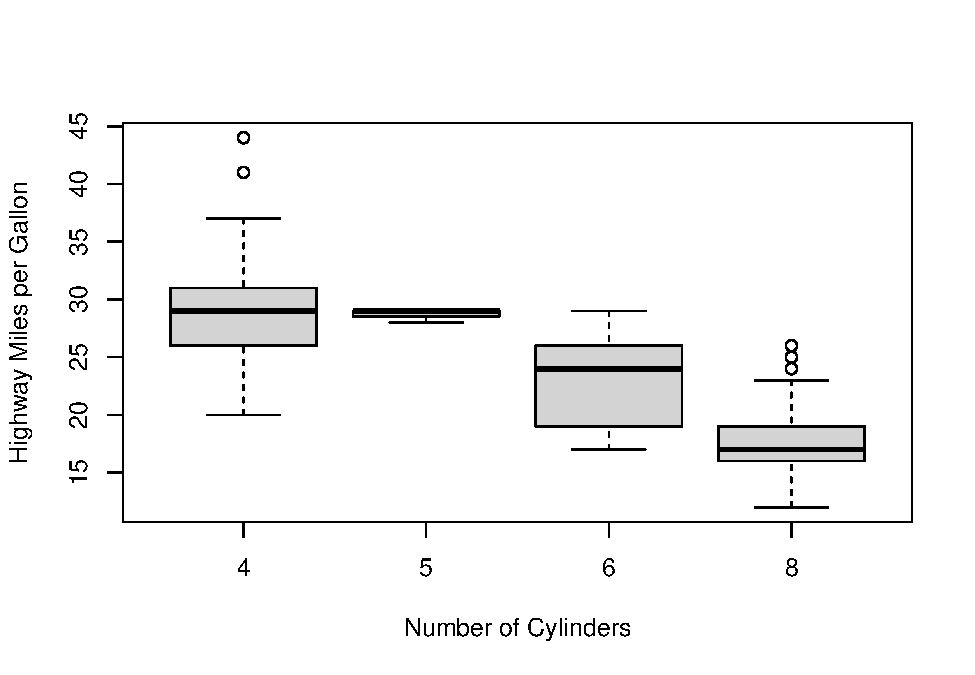
\includegraphics{PSTAT131-HW1_files/figure-latex/unnamed-chunk-4-1.pdf}
Observation: I notice that cars with fewer cylinders can drive more
miles per gallon on highway. In other words, cars with more cylinders
consume more gas.

\textbf{Exercise 5:} Use the corrplot package to make a lower triangle
correlation matrix of the mpg dataset. (Hint: You can find information
on the package here.)

Which variables are positively or negatively correlated with which
others? Do these relationships make sense to you? Are there any that
surprise you?

\begin{Shaded}
\begin{Highlighting}[]
\FunctionTok{library}\NormalTok{(dplyr)}
\FunctionTok{library}\NormalTok{(corrplot)}
\end{Highlighting}
\end{Shaded}

\begin{verbatim}
## corrplot 0.92 loaded
\end{verbatim}

\begin{Shaded}
\begin{Highlighting}[]
\NormalTok{new\_mpg }\OtherTok{\textless{}{-}} \FunctionTok{select}\NormalTok{(mpg,}\SpecialCharTok{{-}}\NormalTok{manufacturer,}\SpecialCharTok{{-}}\NormalTok{model,}\SpecialCharTok{{-}}\NormalTok{trans,}\SpecialCharTok{{-}}\NormalTok{class,}\SpecialCharTok{{-}}\NormalTok{fl,}\SpecialCharTok{{-}}\NormalTok{drv)}
\FunctionTok{corrplot}\NormalTok{(}\FunctionTok{cor}\NormalTok{(new\_mpg), }\AttributeTok{method=}\StringTok{\textquotesingle{}number\textquotesingle{}}\NormalTok{,}\AttributeTok{type=}\StringTok{\textquotesingle{}lower\textquotesingle{}}\NormalTok{)}
\end{Highlighting}
\end{Shaded}

\includegraphics{PSTAT131-HW1_files/figure-latex/unnamed-chunk-5-1.pdf}
Observation of strong positive correlation: cyl and displ, hwy and cty
Observation of strong negative correlation: cty and displ, hwy and
displ, cty and cyl, hwy and cyl Observation of weak positive
correlation: year and displ, cyl and year Observation of weak negative
correlation: cty and year, hwy and year I think this makes sense because
hwy and cty essentially similar to each other, so their correlation with
other variables are quite similar. Moreover, I do not think the year of
manufacturing would have any impact on city mileage or the number of
cylinders that a car has. This also turns out to be true in this
correlation graph.

Exercise 6: Recreate the following graphic, as closely as you can. Hint:
Use the ggthemes package.

\begin{Shaded}
\begin{Highlighting}[]
\FunctionTok{library}\NormalTok{(ggthemes)}
\FunctionTok{library}\NormalTok{(ggplot2)}
\FunctionTok{ggplot}\NormalTok{(mpg, }\FunctionTok{aes}\NormalTok{(}\AttributeTok{x=}\NormalTok{hwy,}\AttributeTok{y=}\NormalTok{class))}\SpecialCharTok{+}\FunctionTok{geom\_boxplot}\NormalTok{()}\SpecialCharTok{+}\FunctionTok{labs}\NormalTok{(}\AttributeTok{x=}\StringTok{"Highway MPG"}\NormalTok{,}\AttributeTok{y=}\StringTok{"Vehnicle Class"}\NormalTok{)}\SpecialCharTok{+}\FunctionTok{theme\_gdocs}\NormalTok{()}\SpecialCharTok{+}\FunctionTok{geom\_jitter}\NormalTok{(}\AttributeTok{alpha =} \FloatTok{0.2}\NormalTok{) }
\end{Highlighting}
\end{Shaded}

\includegraphics{PSTAT131-HW1_files/figure-latex/unnamed-chunk-6-1.pdf}

Exercise 7 Recreate the following graphic.

\begin{Shaded}
\begin{Highlighting}[]
\FunctionTok{ggplot}\NormalTok{(mpg, }\FunctionTok{aes}\NormalTok{(}\AttributeTok{x=}\NormalTok{class,}\AttributeTok{y=}\NormalTok{hwy,}\AttributeTok{fill=}\NormalTok{drv))}\SpecialCharTok{+}\FunctionTok{geom\_boxplot}\NormalTok{()}\SpecialCharTok{+}\FunctionTok{labs}\NormalTok{(}\AttributeTok{x=}\StringTok{"class"}\NormalTok{,}\AttributeTok{y=}\StringTok{"hwy"}\NormalTok{)}\SpecialCharTok{+}\FunctionTok{scale\_color\_calc}\NormalTok{()}
\end{Highlighting}
\end{Shaded}

\includegraphics{PSTAT131-HW1_files/figure-latex/unnamed-chunk-7-1.pdf}

Exercise 8 Recreate the following graphic.

\begin{Shaded}
\begin{Highlighting}[]
\FunctionTok{ggplot}\NormalTok{(mpg,}\FunctionTok{aes}\NormalTok{(}\AttributeTok{x=}\NormalTok{displ,}\AttributeTok{y=}\NormalTok{hwy))}\SpecialCharTok{+}\FunctionTok{geom\_point}\NormalTok{(}\FunctionTok{aes}\NormalTok{(}\AttributeTok{color=}\NormalTok{drv))}\SpecialCharTok{+}\FunctionTok{labs}\NormalTok{(}\AttributeTok{x=}\StringTok{"displ"}\NormalTok{,}\AttributeTok{y=}\StringTok{"hwy"}\NormalTok{)}\SpecialCharTok{+}\FunctionTok{scale\_shape\_stata}\NormalTok{()}\SpecialCharTok{+}\FunctionTok{geom\_smooth}\NormalTok{(}\AttributeTok{se =} \ConstantTok{FALSE}\NormalTok{,}\FunctionTok{aes}\NormalTok{(}\AttributeTok{linetype=}\NormalTok{drv))}
\end{Highlighting}
\end{Shaded}

\begin{verbatim}
## `geom_smooth()` using method = 'loess' and formula 'y ~ x'
\end{verbatim}

\includegraphics{PSTAT131-HW1_files/figure-latex/unnamed-chunk-8-1.pdf}

\end{document}
